\documentclass[12pt,german,a4paper]{scrreprt}

\usepackage[ngerman]{babel}
\usepackage[utf8]{inputenc} 
\usepackage{lmodern}
\usepackage{listings}
\usepackage{color}
\usepackage{amsmath}
\usepackage{amssymb}
\usepackage{pdfpages}
\usepackage{geometry}
\geometry{a4paper, left=1.5cm,right=1.5cm, top=2cm, bottom=2cm} 

\title{Skript Numerische Methoden I}
\subtitle{Finite-Elemente-Methoden und Randelemente-Methoden}
\author{Christian Kroh}
\date{\today{}, Dresden}

\begin{document}
\maketitle
\newpage
\tableofcontents
\newpage
\part{Randwertaufgaben (RWA)}
\newpage
\chapter{Formulierung und näherungsweise Lösung von Randwertaufgaben (RWA)}
\section{Randwertaufgabe (RWA)}
\begin{itemize}
\item besteht aus 
	\begin{itemize}
	\item \textbf{Differentialgleichung (DGL)}\\
		\(\underline{D}(\underline{u}(\underline{x})) + \underline{\rho}(\underline{x}) = \underline{0} \qquad \forall x \in \Omega\)
	
	\item \textbf{Randbedingungen (RB)}\\
		\(\underline{D_1}(\underline{u}(\underline{x})) + \underline{r_1}(\underline{x}) = \underline{0} \qquad \forall x \in \Gamma_1\)
		
	\item \textbf{Differentialoperatoren}\\
		\(\underline{D}(...), (\underline{D_1}(...), (\underline{D_2}(...), ...\) Differentialoperatoren
	\item \(\underline{x}\) ... Ortsvektor
	\item \(\underline{\rho}, \underline{r_i}\) ... rechte Seite
	\item \(\Gamma_1\) ... Rand mit \underline{wesentlichen} Randbedingungen
	\item \(\Gamma_2\) ... Rand mit \underline{natürlichen} Randbedingungen\\
		\(\Gamma_1 \cup \Gamma_2 = \Gamma; \Gamma_1 \cap \Gamma_2 = \emptyset\)\\
		(für jede Koordinatenwichtung)
	\end{itemize}
	\item analytische Lösung nur für einfache Problemstellungen 
	\item Annahme: 
		\begin{itemize}
		\item kinematische Annahmen (Bernoulli)
		\item kinetische Annahmen
		\end{itemize}
\end{itemize}


\section{Formulierung der Randwertaufgabe}
Beispiel Zugstab\\
(Graphik Zugstab einfügen)\\
\subsection{Differentielle Formulierung}
Auswertung von Bilanzgleichungen an einem infinitessimalen Volumenelement\\
\begin{itemize}
\item Gleichgewichtsbedingung: \\
\(\downarrow -F_L + F_L + dF_L + q\,dx = 0 \\\\ \frac{dF_L}{dx} = -q \\\\ F_L' = -q\)

\item kinetische Annahme:\\
	\(F_L = \sigma \cdot A \)
	
\item kinematische Annahme\\
	\(\epsilon = \frac{du}{dx} = u'\)
	
\item[$\Rightarrow$] konstitutive Beziehung (Material)\\
	\(\sigma = E \cdot \epsilon\)
	
\item[$\Rightarrow$] Einsetzen in die Grundgleichung\\
	\(F_L = \sigma \cdot A = E \cdot \epsilon \cdot A \quad \Rightarrow \quad F_L' = (E \cdot A \cdot u')' = -q\)
\end{itemize}
\paragraph{Annahme: konstanter Querschnitt}\hfill\\\\
\(E\,A\,u'' + q = 0 \qquad \forall x \in [0,l]\)

\begin{description}
	\item[Randbedingungen]\hfill
		\begin{itemize}
		\item wesentliche RB: \(u(x=0) = \tilde{u} = 0 \)
		\item natürliche RB: \(F_L (x=l) = F = 0 \\ E\,A\,u' (x=l) = F = 0\)
		\end{itemize}
	\item[Zuordnung]\hfill\\
			\(D = E\,A (...)'' \\
			D_1 = 1 (...) \\
			D_2 = E\,A(...)' \\
			\Omega : x \in [0, l] \\
			\Gamma_1 : x = 0 \\
			\Gamma_2 : x = l \)
\end{description}

\subsection{Variationsformulierung}
\begin{description}
	\item[Grundlage : Variationsrechnung] Verformung eines elastischen Systems, sodass eleastisches Gesamtpotential extremal (Minimum)
	
	\item[Voraussetzungen:]\hfill \\
		\begin{itemize}
			\item elastisches Materialverhalten\\
			\(\Gamma = \frac{d \Pi_i}{d \epsilon}\)
			\item Potential der äußeren Lasten \\
			\(F = \frac{d \Pi_\epsilon}{d u}\)
		\end{itemize}
	\item[Variationsformulierung für Mechanik] Prinzip vom stationären Wert des elastischen Gesamtsystems \\\\ Vorgaben zur Herleitung der DGL und RB:
		\begin{itemize}
			\item Aufstellen des elastischen Gesamtpotentialfelds
			\item suchen des stationären Werts $\Pi \rightarrow$ min, max
		\end{itemize}
	\item[Kontinuum] funktional d.h. Funktion von Funktionen\\
		\(\Pi = \Pi (u (x) , u' (x), x) \rightarrow min, max\)
		
	\item[notwendige Bedingung] für stionären Wert (Extremwert)\\
		\(d \,\Pi = 0\) \hspace{2cm} $d \,\Pi$ ... erste Variation von $\Pi$\\
		\paragraph{Bsp: Stabproblem - Aufstellen des Potentials}\hfill \\
		\(	\Pi = \Pi_i - \Pi_a\\
			\Pi_i = \Pi_f\) ... Veränderungspotential\\
		\(	\Pi_i = \int\limits_\Omega \Pi_i^* \, dV\)
\end{description}

\subsection{Prinzip der virtuellen Arbeit}
\begin{itemize}
	\item elektrisches Gesamtpotential: Einschränkung auf elastische Potentiallasten
	\item[$\Rightarrow$] Prinzip der virtuellen Arbeit ist allgemein anwendbar = Prinzip der virtuellen Verschiebung
	
	\begin{itemize}
		\item virtuelle Arbeit {\boldmath\(\partial W\)} wird an einem System verrichtet (durch eine geringfügige Störung \(\partial u\) des Verschiebungsfeldes \(u\))
		\item Eigenschaften von \textbf{\boldmath\(\partial u\) = virtuelle Verschiebung}
			\begin{itemize}
				\item beliebig
				\item infinitessimal
				\item kinematisch zulässig (\(\partial u = 0\))
			\end{itemize}
		\item Gleichgewicht (GGW) entspricht der Forderung \\
			\(\partial W = 0\)\\
			\(\partial W = \partial W_{innen} + \partial W_{außen} = 0\)
	\end{itemize}
\end{itemize}
\paragraph{Beispiel: Stab}
	\(\partial W = \int G \partial \rho\,dV - \int\limits_0^l q\,du\,dx - Fdu(l)\)\\
	beliebiges Materialverhalten, keine Einschränkungen\\
	\(\Rightarrow\) GGW: \(\partial W = 0\)\\
	\(\Gamma = E \epsilon\), \(\epsilon = u'\), \(dV = Ad\)\\\\
	{\boldmath\(\partial W = \int\limits_0^l EAu' \partial u'\, dx - \int\limits_0^l q \partial u\, dx - Fdu(l) = 0\)}\\\\
	$\Rightarrow$ partielle Integration, \(\partial u(0) = 0\), sonst \(\partial u\) beliebig\\
	liefert 
	\begin{itemize}
		\item \(E A u'' + q = 0 \qquad\) DGL
		\item \(E A u'(l) -F = 0 \qquad\) natürliche Randbedingung
	\end{itemize}

\section{Näherungsweises Lösen einer RWA}
\textbf{Methode der gewichteten Residuen}
\begin{itemize}
\item Ansatz für Feldvariable, z.B. Verschiebung\\
	\(u(x) \sim \tilde{u} (x)\\\tilde{u}(x) = \sum\limits_{i=1}^n g_i(x)\,u_i\)\\
	$g_i$ ... Basisfunktion\\
	$u_i$ ... Ansatzfreiwerte
\item DGL und RB werden im Ansatz nicht mehr exakt ermittelt\\
	$\Rightarrow$ Residuen $\eta_i (x)$\\\\
	\(D( \tilde{u} (x)) + \rho (x) = \eta (x) \neq 0 \qquad \forall x \in \Gamma \\
	D_1 (\tilde{u}(x)) + r_1 (x) = \eta_1 ( x) \neq 0 \qquad \forall x \in \Gamma_1 \\
	D_L (\tilde{u} (x)) + r_L (x) = \eta_L (x) \neq 0 \qquad \forall x \in \Gamma_L\) 
	\begin{itemize}
	\item Multiplikation der Residuen der DGL $\eta (x)$
	\item[$\Rightarrow$] Näherungslösung erfüllt Forderung	\(\int\limits_W \eta (x)\, w(x) \, dx = 0\) 
	\item Ziel: GLS zur Berechnung der Freiwerte $u_i$
	\item Verfahren definiert durch:
		\begin{itemize}
		\item Form der gewichteten Residuen
		\item Wahl der Wichtungsfunktion
		\end{itemize}
	
	\end{itemize}
\end{itemize}

\subsection{Starke Form}
{\boldmath\(\int\limits_0^l \eta (x) \, w(x) \, dx = 0\)}\\\\
\textbf{Beispiel: Zugstab}\\
\begin{itemize}
\item Voraussetzungen: Ansatz ...\\
	\begin{itemize}
	\item zweimal stetig (nicht trivial) differenzierbar
	\item alle Randbedingungen (\(\eta_1 = 0,\, \eta_2 = 0\))
	\item[$\Rightarrow$] starke Form 
	\end{itemize}
\item GLS für Freiwerte $u_i$\\
	$\Rightarrow$ verschiedenste Lösungsverfahren, durch unterschiedliche Wahl der Wichtungsfunktion $u(x)$ (z.B. Kollokation, Methode der Momente, Galerkin Verfahren, Minimum des Fehlerquadratintegrals)\\
	\textbf{Besipiel: DIRAC-Funktion (Kollokation)}\\
	\(W(x) = \partial (x - \xi_i) \qquad \partial = \left\{\begin{array}{l l} \infty \quad x = \xi \\ 0 \quad \text{sonst} \end{array} \right. \\ \int \eta (x) \, \partial (x - \xi)\,dx = \eta (\rho)\)
\end{itemize}


\includepdf[pages={10-12}, scale=1, pagecommand={}, nup=1x3]{RWA/refs/NM_VL_2_2013_10_23.pdf}

\newpage
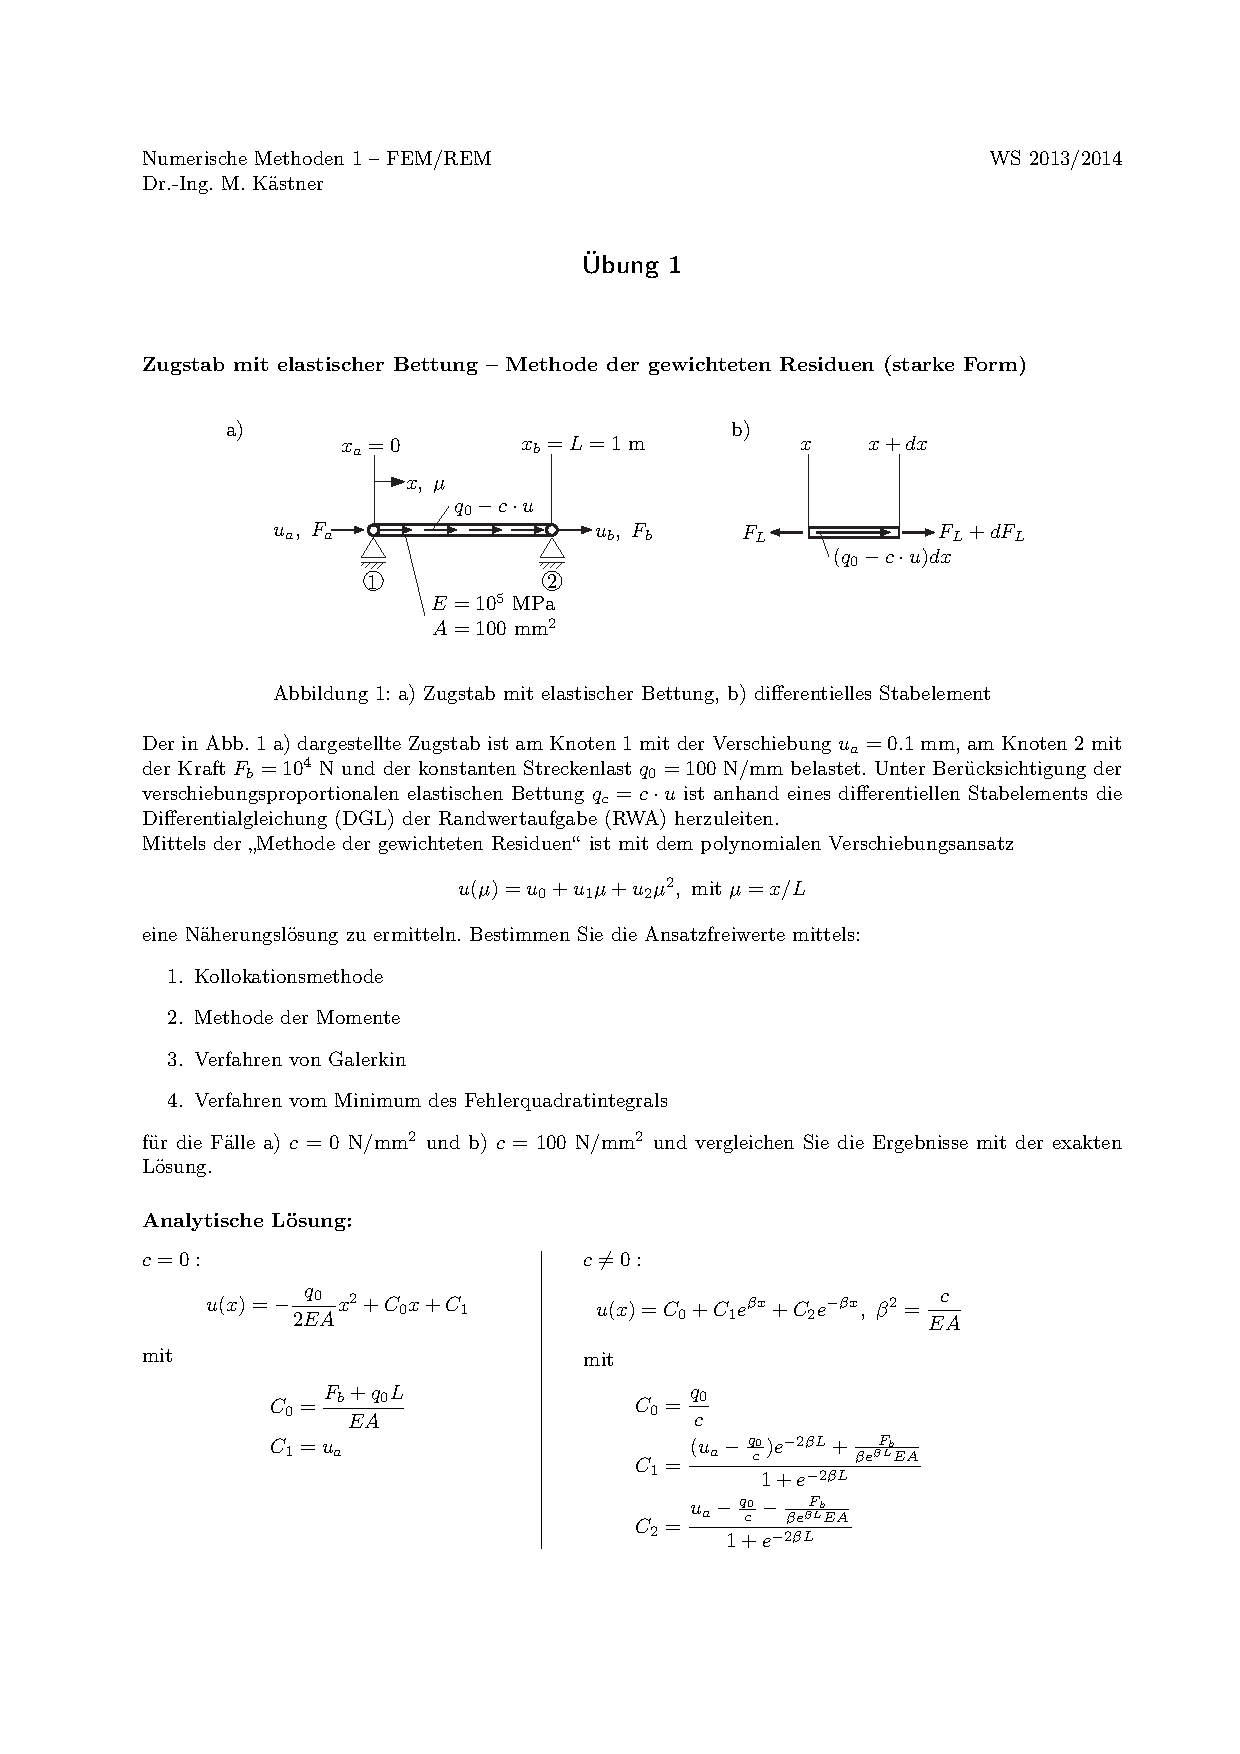
\includepdf[pages={1}, scale=0.9,  pagecommand=\section{Übung 1}]{RWA/refs/NM1_Uebung01_Aufgabe_2013.pdf}
\section{Übung 1 - Lösung}
usw.



\part{Einführung in die Finite-Elemente-Methode (FEM)}
\newpage
\input{FEM/00-FEM}

\part{Einführung in die Randelemente-Methode (REM)}
\newpage
\input{REM/00-REM}
\end{document}
